%
% 
 % Sarang Bhadsavle (ssb2243)
 % EE382C: Multicore Computing
 % Scribe Notes for Lecture 6 (09/13/2016)

% This is the LaTeX template file for lecture notes for EE 382C/EE 361C.
% To familiarize yourself with this template, the body contains
% some examples of its use.  Look them over.  Then you can
% run LaTeX on this file.  After you have LaTeXed this file then
% you can look over the result either by printing it out with
% dvips or using xdvi.
%
% This template is based on the template for Prof. Sinclair's CS 270.

\documentclass[twoside]{article}
%\usepackage{graphics}
\usepackage{graphicx}
\usepackage{amsmath}
\usepackage{amssymb}
\usepackage{algorithm}
\usepackage[noend]{algpseudocode}
\setlength{\oddsidemargin}{0.25 in}
\setlength{\evensidemargin}{-0.25 in}
\setlength{\topmargin}{-0.6 in}
\setlength{\textwidth}{6.5 in}
\setlength{\textheight}{8.5 in}
\setlength{\headsep}{0.75 in}
\setlength{\parindent}{0 in}
\setlength{\parskip}{0.1 in}

%
% The following commands set up the lecnum (lecture number)
% counter and make various numbering schemes work relative
% to the lecture number.
%
\newcounter{lecnum}
\renewcommand{\thepage}{\thelecnum-\arabic{page}}
\renewcommand{\thesection}{\thelecnum.\arabic{section}}
\renewcommand{\theequation}{\thelecnum.\arabic{equation}}
\renewcommand{\thefigure}{\thelecnum.\arabic{figure}}
\renewcommand{\thetable}{\thelecnum.\arabic{table}}

%
% The following macro is used to generate the header.
%
\newcommand{\lecture}[4]{
   \pagestyle{myheadings}
   \thispagestyle{plain}
   \newpage
   \setcounter{lecnum}{#1}
   \setcounter{page}{1}
   \noindent
   \begin{center}
   \framebox{
      \vbox{\vspace{2mm}
    \hbox to 6.28in { {\bf EE 382C/361C: Multicore Computing
                        \hfill Fall 2016} }
       \vspace{4mm}
       \hbox to 6.28in { {\Large \hfill Lecture #1: #2  \hfill} }
       \vspace{2mm}
       \hbox to 6.28in { {\it Lecturer: #3 \hfill Scribe: #4} }
      \vspace{2mm}}
   }
   \end{center}
   \markboth{Lecture #1: #2}{Lecture #1: #2}
   %{\bf Disclaimer}: {\it These notes have not been subjected to the
   %usual scrutiny reserved for formal publications.  They may be distributed
   %outside this class only with the permission of the Instructor.}
   \vspace*{4mm}
}

%
% Convention for citations is authors' initials followed by the year.
% For example, to cite a paper by Leighton and Maggs you would type
% \cite{LM89}, and to cite a paper by Strassen you would type \cite{S69}.
% (To avoid bibliography problems, for now we redefine the \cite command.)
% Also commands that create a suitable format for the reference list.
\renewcommand{\cite}[1]{[#1]}
\def\beginrefs{\begin{list}%
        {[\arabic{equation}]}{\usecounter{equation}
         \setlength{\leftmargin}{2.0truecm}\setlength{\labelsep}{0.4truecm}%
         \setlength{\labelwidth}{1.6truecm}}}
\def\endrefs{\end{list}}
\def\bibentry#1{\item[\hbox{[#1]}]}

%Use this command for a figure; it puts a figure in wherever you want it.
%usage: \fig{NUMBER}{SPACE-IN-INCHES}{CAPTION}
\newcommand{\fig}[3]{
			\vspace{#2}
			\begin{center}
			Figure \thelecnum.#1:~#3
			\end{center}
	}
% Use these for theorems, lemmas, proofs, etc.
\newtheorem{theorem}{Theorem}[lecnum]
\newtheorem{lemma}[theorem]{Lemma}
\newtheorem{proposition}[theorem]{Proposition}
\newtheorem{claim}[theorem]{Claim}
\newtheorem{corollary}[theorem]{Corollary}
\newtheorem{definition}[theorem]{Definition}
\newenvironment{proof}{{\bf Proof:}}{\hfill\rule{2mm}{2mm}}

% **** IF YOU WANT TO DEFINE ADDITIONAL MACROS FOR YOURSELF, PUT THEM HERE:

\algdef{SE}[SUBALG]{Indent}{EndIndent}{}{\algorithmicend\ }%
\algtext*{Indent}
\algtext*{EndIndent}

\makeatletter
\def\BState{\State\hskip-\ALG@thistlm}
\makeatother

\begin{document}
%FILL IN THE RIGHT INFO.
%\lecture{**LECTURE-NUMBER**}{**DATE**}{**LECTURER**}{**SCRIBE**}
\lecture{6}{September 13}{Vijay Garg}{Sarang Bhadsavle}
%\footnotetext{These notes are partially based on those of Nigel Mansell.}

% **** YOUR NOTES GO HERE:

% Some general latex examples and examples making use of the
% macros follow.  
%**** IN GENERAL, BE BRIEF. LONG SCRIBE NOTES, NO MATTER HOW WELL WRITTEN,
%**** ARE NEVER READ BY ANYBODY.
\section*{Agenda and Announcements}
Today's lecture covered the following topics:
\begin{itemize}
  \item The lower bound on the number of shared locations required for mutual exclusion
  \item Fischer's Algorithm (A timing-based algorithm)
  \item Lamport's Fast Mutex Algorithm
  \begin{itemize}
	\item Splitter Construct
  \end{itemize}
\end{itemize}

Additionally, remember to watch the video seminar \textit{Toward Extreme-Scale Manycore Architectures} 
and the video lectures on Semaphores from last week, as they will be covered on the first exam.

\section{Lower Bound on Number of Shared Locations}

Question: Is there any algorithm which, by using just one shared variable, we can achieve mutual exclusion?

\begin{definition}{Covering State}

The notion of a state in which all shared variables are about to be overwritten by processes and the shared state is consistent with no process in the critical section.
\end{definition}

\begin{theorem}
(Barnes and Lynch) Any mutex algorithm that only uses read-write variables on \textit{n} processes requires at least \textit{n} shared locations.
\end{theorem}

\begin{proof}
(n = 2)

Let P and Q be processes and let A be a shared memory location whose initial value is $\bot$. Let Q run until it is about to write to A, i.e. it is in the Covering State. Now let P run and enter the critical section. Let Q run again. Q writes to A and enters the critical section. 

$\therefore$ Two processes are simultaneously in the critical section

$\therefore$ Violation of mutual exclusion
\end{proof}

This proof can be extended to \textit{n} \textgreater \ 2 by following a similar sequence of events to achieve a Covering State, and then letting processes run and enter the critical section simultaneously, causing a violation of mutual exclusion.

\section{Fischer's Algorithm}

It is possible to achieve mutual exclusion of \textit{n} processes with a single shared variable, provided that a key assumption is made about the timing of the algorithm. The algorithm along with this assumption is shown below.

\begin{algorithm}
\caption{Fischer's Algorithm (for a process ${P_i}$)}\label{fischers}
\begin{algorithmic}[1]
\State \text{shared var} \textit{turn}  \text{= -1;} // door is open \newline
\Procedure{requestCS}{}
\State \emph{while(true):}
\Indent
	\State \emph{while(turn != -1):}
    \Indent
		\State $ \text{noOp(); }$
    \EndIndent
    \State \textit{turn} \text{=} \textit{i;}
    \State \text{wait for} \textit{$\bigtriangleup$t} \text{time units;}
    \State \emph{if(turn == i):}
    \Indent 
    	\State \text{return;}
    \EndIndent 
\EndIndent 
\EndProcedure \newline

\Procedure{releaseCS}{}
\State \textit{turn} \text{= -1;}
% \BState \emph{top}:
% \If {$i > \textit{stringlen}$} \Return false
% \EndIf
% \State $j \gets \textit{patlen}$
% \BState \emph{loop}:
% \If {$\textit{string}(i) = \textit{path}(j)$}
% \State $j \gets j-1$.
% \State $i \gets i-1$.
% \State \textbf{goto} \emph{loop}.
% \State \textbf{close};
% \EndIf
% \State $i \gets i+\max(\textit{delta}_1(\textit{string}(i)),\textit{delta}_2(j))$.
% \State \textbf{goto} \emph{top}.
\EndProcedure
\end{algorithmic}
\end{algorithm}

The key assumption with Fischer's Algorithm is that $\bigtriangleup$t $\ge$ \textit{c}, where \textit{c} is is the maximum time required to close the door i.e. the time required to set \textit{turn} to \textit{i}.

Without this assumption, the following sequence of events could occur and cause a violation of mutual exclusion for two processes, ${P_i}$ and ${P_j}$:
\begin{enumerate}
  \item ${P_i}$ reads turn = -1
  \item ${P_j}$ reads turn = -1
  \item ${P_j}$ sets turn = j
  \item ${P_j}$ reads turn = j, and enters critical section
  \item ${P_i}$ sets turn = i
  \item ${P_i}$ reads turn = i and enters critical section
\end{enumerate}

Fischer's algorithm satisfies mutex by ensuring that the time period that a process ${P_j}$ waits after setting turn = j and before checking if turn == j is greater than the time period that another process ${P_i}$ takes after reading turn == -1 and before setting turn = i. This ensures that only one process (in this case, ${P_i}$) can enter the critical section.

\section{Lamport's Fast Mutex Algorithm}

Lamport's Fast Mutex Algorithm is used to provide mutual exclusion in a very fast way when there is no contention for the critical section. When there is contention, the regular method of mutual exclusion is followed.

\subsection*{Splitter}

The construct of a "splitter" is used in Lamport's Fast Mutex algorithm, as seen in Figure \ref{fig:splitter}.

\begin{figure}
\centering
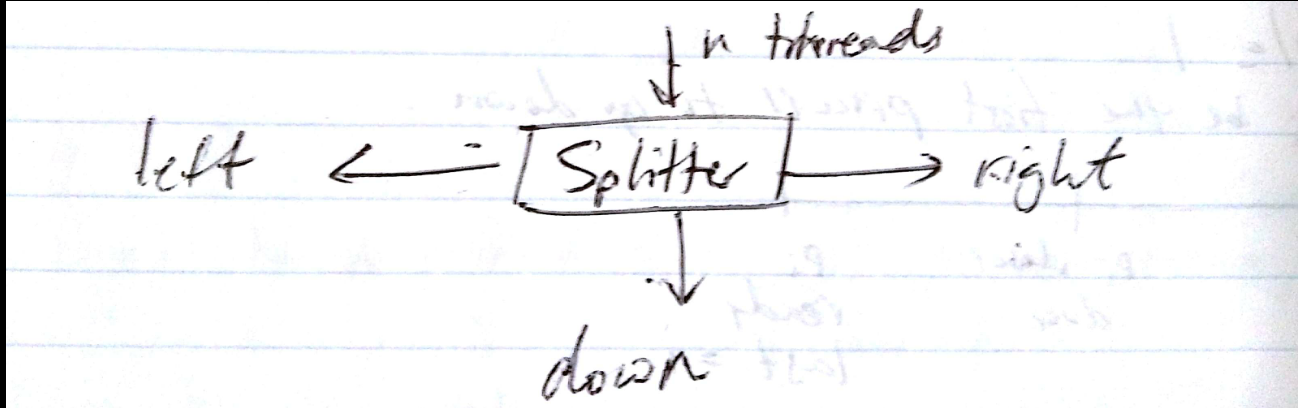
\includegraphics[width=0.9\textwidth]{Screenshot_20160918-185557.png}
\caption{\label{fig:splitter}A Splitter Construct}
\end{figure}

The Splitter guarantees that:

\begin{itemize}
  \item The number of processes sent right $\le$ n - 1
  \item The number of processes sent left $\le$ n - 1
  \item The number of processes sent down $\le$ 1
\end{itemize}

\begin{algorithm}
\caption{Splitter Construct (for a process ${P_i}$)}\label{splitterConstruct}
\begin{algorithmic}[1]
\State \text{shared var} \textit{door}  \text{: $\{open, closed\}$} \textit{init} \text{open;}
\State \text{shared var} \textit{last}  \text{: pid} \textit{init} \text{-1;}\newline

\State \textit{last} \text{=} \textit{i;}
\State \emph{if(door == closed):}
\Indent
	\State \text{return} \textit{left;}
\EndIndent
\State \emph{else:}
\Indent
	\State \textit{door} \text{=} \textit{closed;}
    \State \emph{if(last == i):} \text{return} \textit{down;}
    \State \emph{else:} \text{return} \textit{right;}
\EndIndent
\end{algorithmic}
\end{algorithm}

\begin{claim}
$\|$left$\|$ $\le$ n - 1
\end{claim}
\begin{proof}
Some process \emph{must} have closed the door.
\end{proof}

\begin{claim}
$\|$right$\|$ $\le$ n - 1
\end{claim}
\begin{proof}
Consider the process ${P_i}$ such that textit{last} = textit{i}. Then ${P_i}$ must be  part of left or down.
\end{proof}

\begin{claim}
$\|$down$\|$ $\le$ 1
\end{claim}
\begin{proof}
Let a process ${P_i}$ be the first process to go down. In order to go down, ${P_i}$ must execute 3 steps:
\begin{enumerate}
\item ${P_i}$ writes \textit{last} \label{pf1}
\item ${P_i}$ closes \textit{door} \label{pf2}
\item ${P_i}$ reads \textit{last == i} \label{pf3}
\end{enumerate}
Suppose there is some other process ${P_j}$ also in the splitter. ${P_i}$ must write \textit{last} at some point. There are 3 cases:

\begin{itemize}

\item Suppose ${P_j}$ writes \textit{last} before \ref{pf1}. Then ${P_j}$ would be the first process to go down, which violates the initial supposition that ${P_i}$ went down first 


\item Suppose ${P_j}$ writes \textit{last} after \ref{pf1} but before \ref{pf3}. However, this is not possible because ${P_i}$ read \textit{last == i}.


\item Suppose ${P_j}$ writes \textit{last} after \ref{pf3}. However, this is not possible because ${P_j}$ could not have found \textit{door} to be open in the first place.
    
\end{itemize}
$\therefore$ Since all 3 cases are shown to be impossible, there can only be at most one process that goes down in the Splitter.
\end{proof}

Lamport's Fast Mutex algorithm can be constructed using Splitter, as seen in Figure \ref{fig:lamportfast}.

\begin{figure}
\centering
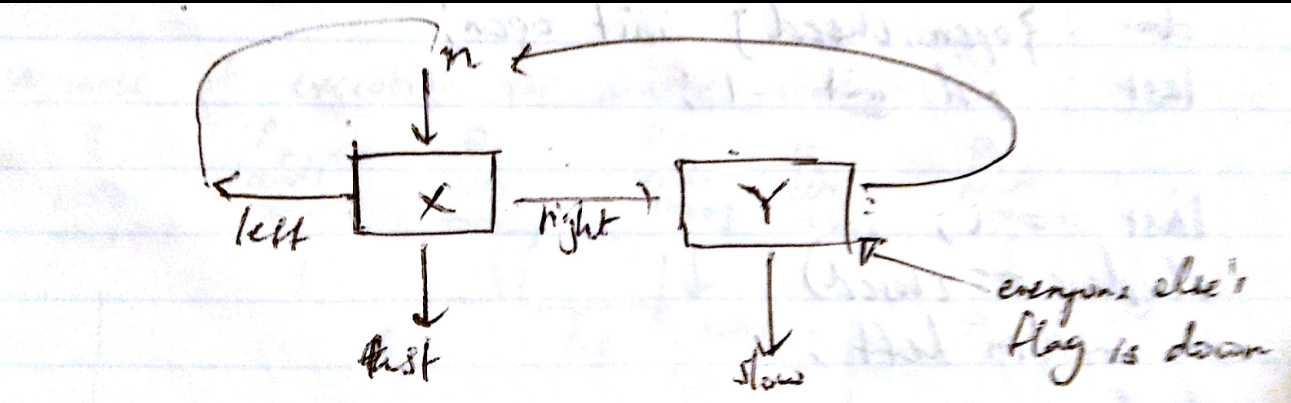
\includegraphics[width=0.9\textwidth]{lamportfast.png}
\caption{\label{fig:lamportfast}Design of Lamport's Fast Mutex Algorithm using Splitter}
\end{figure}

\begin{algorithm}
\caption{Lamport's Fast Mutex Algorithm (for a process ${P_i}$)}\label{lamportFast}
\begin{algorithmic}[1]
\Procedure{acquire}{}
\State \emph{while(true):}
\Indent
	\State \textit{flag[i]} \text{=} \textit{up;}
    \State \textit{x} \text{=} \textit{i;}
    \State \emph{if(y != i):} \text{// splitter's left}
	\Indent
		\State \textit{flag[i]} \text{=} \textit{down;}
        \State \emph{waitUntil(y == -1):}
        \State \text{continue;}
	\EndIndent
    \State \emph{else:}
    \Indent
    	\State \textit{y} \text{=} \textit{i;}
        \State \emph{if(x == i):} \text{return; // fast path}
        \State \emph{else:} \text{// splitter's right}
        \Indent 
        	\State \textit{flag[i]} \text{=} \textit{down;}
            \State \emph{waitUntil($\forall$j : flag[j] == down);}
            \State \emph{if(y == i):} \text{return; // slow path}
            \State \emph{else:}
            \Indent
            	\State \emph{waitUntil(y == -1);}
                \State \text{continue;}
            \EndIndent
        \EndIndent 
    \EndIndent 
\EndIndent
\EndProcedure \newline

\Procedure{release}{}
	\State \textit{y} \text{=} \textit{-1;}
    \State \textit{flag[i]} \text{=} \textit{down;}
\EndProcedure

\end{algorithmic}
\end{algorithm}

\begin{proposition}
Note that Lamport's Fast Mutex Algorithm does not guarantee starvation-freedom
\end{proposition}

\clearpage

\section*{References}
\beginrefs
\bibentry{1}{\sc Vijay Garg.}
EE382C, Multicore Computing, The University of Texas at Austin. September 2016.
\endrefs



\end{document}





